\documentclass[14pt,aspectratio=1610]{beamer}

\usepackage[brazil]{babel}
\usepackage[utf8]{inputenc}
%\UseRawInputEncoding
\usepackage[T1]{fontenc}
%\usepackage{Sweave}
\usepackage{animate}
\usepackage{amsbsy}
\usepackage{amsfonts}
\usepackage{amsmath}
\usepackage{amssymb}
\usepackage{amsthm}
\usepackage[toc,page,title,titletoc]{appendix}
%\usepackage[fixlanguage]{babelbib}
%\usepackage[pdftex]{color}
\usepackage{dsfont}
\usepackage{esvect}
\usepackage[labelfont=bf]{caption}
\usepackage{subcaption}
\usepackage{float}
\usepackage[Glenn]{fncychap}%Sonny %Conny %Lenny %Glenn %Renje %Bjarne %Bjornstrup
%\usepackage{geometry, calc, color, setspace}%
%\geometry{a4paper, headsep=1.0cm, footskip=1cm, lmargin=3cm, rmargin=2cm, tmargin=3cm, bmargin=2cm}
\usepackage{graphicx}
\usepackage{indentfirst}%Para indentar os parágrafos automáticamente
\usepackage{lipsum}
\usepackage{longtable}
\usepackage{mathtools}
\usepackage{listings}%Inserir codigo do R no latex
\usepackage{multirow}
\usepackage{multicol}
\usepackage{csquotes}
\usepackage[maxcitenames=2,terseinits=true,natbib=true, style=authoryear, maxbibnames=99]{biblatex}
\addbibresource{../Referencias/Referencias.bib}
%\usepackage{csquotes}
%\usepackage[natbib=true,style=abnt, sorting=none]{biblatex}
%\addbibresource{bibliografia.bib}
\usepackage[figuresright]{rotating}
\usepackage{spalign}
%\usepackage{pgfpages}
\usepackage{pgfplots}
\pgfplotsset{compat=1.18}
\usepackage{tikz}
\usepackage{color, colortbl}
\usepackage{ragged2e}%para justificar o texto dentro de algum ambiente
\definecolor{Gray}{gray}{0.9}
\definecolor{LightCyan}{rgb}{0.88,1,1}
%\usepackage{grffile}

\usepackage[all]{xy}



%\usetheme{Madrid}
%\usecolortheme[RGB={193,0,0}]{structure}
\usetheme{metropolis}
\definecolor{mycolor}{RGB}{34, 45, 50}
\setbeamercolor{structure}{fg=mycolor}
\usepackage{mathpazo} % Fonte elegante para matemática
\usepackage{helvet} % Fonte sans-serif para texto
\renewcommand{\familydefault}{\sfdefault} % Definir fonte padrão como sans-serif

%\setbeamertemplate{footline}[frame number]
%\setbeamertemplate{footline}[text line]{%
%  \parbox{\linewidth}{\vspace*{-8pt}\hfill\date{}\hfill\insertshortauthor\hfill\insertpagenumber}}
\beamertemplatenavigationsymbolsempty
\renewcommand{\vec}[1]{\mbox{\boldmath$#1$}}
\newtheorem{Teorema}{Teorema}
\newtheorem{Proposicao}{Proposição}
\newtheorem{Definicao}{Definição}
\newtheorem{Corolario}{Corolário}
\newtheorem{Demonstracao}{Demonstração}
\newcommand{\bx}{\ensuremath{\bar{x}}}
\newcommand{\Ho}{\ensuremath{H_{0}}}
\newcommand{\Hi}{\ensuremath{H_{1}}}


\apptocmd{\frame}{}{\justifying}{} % Allow optional arguments after frame.

\title{Estatística I}
\author{Prof. Fernando de Souza Bastos \texorpdfstring{\\ fernando.bastos@ufv.br}{}}
\institute{Departamento de Estatística \texorpdfstring{\\ Universidade Federal de Viçosa}{}\texorpdfstring{\\ Campus UFV - Viçosa}{}}
\date{}
\newcommand\mytext{Aula 5}
\newcommand\mytextt{Fernando de Souza Bastos}
\newcommand\mytexttt{\url{https://ufvest.github.io/}}

\makeatletter
\setbeamertemplate{footline}
{
  \leavevmode%
  \hbox{%
  \begin{beamercolorbox}[wd=.3\paperwidth,ht=2.25ex,dp=1ex,center]{author in head/foot}%
    \usebeamerfont{author in head/foot}\mytext
  \end{beamercolorbox}%
  \begin{beamercolorbox}[wd=.3\paperwidth,ht=2.25ex,dp=1ex,center]{title in head/foot}%
    \usebeamerfont{title in head/foot}\mytextt
  \end{beamercolorbox}%
  \begin{beamercolorbox}[wd=.35\paperwidth,ht=2.25ex,dp=1ex,right]{site in head/foot}%
    \usebeamerfont{site in head/foot}\mytexttt\hspace*{2em}
    \insertframenumber{} / \inserttotalframenumber\hspace*{2ex} 
  \end{beamercolorbox}}%
  \vskip0pt%
}
\makeatother

\providecommand{\arcsin}{} \renewcommand{\arcsin}{\hspace{2pt}\textrm{arcsen}}
\providecommand{\sin}{} \renewcommand{\sin}{\hspace{2pt}\textrm{sen}}
%\newtheorem{Teorema}{Teorema}
%\newtheorem{Proposicao}{Proposição}
%\newtheorem{Definicao}{Definição}
%\newtheorem{Corolario}{Corolário}
%\newtheorem{Demonstracao}{Demonstração}

\titlegraphic{\hspace*{8cm}\href{https://fsbmat-ufv.github.io/}{
\includegraphics[width=2cm]{figs/mylogo.png}}
}


\usepackage{hyperref,bookmark}
\hypersetup{
  colorlinks=true,
  linkcolor=blue,
  citecolor=red,
  filecolor=blue,
  urlcolor=blue,
}

% Layout da pagina
\hypersetup{pdfpagelayout=SinglePage}
\begin{document}
%\Sconcordance{concordance:Aula5.tex:Aula5.Rnw:%
1 209 1 1 15 1 2 8 1 1 15 1 2 8 1 1 12 1 2 27 1 1 21 1 2 41 1 1 16 1 2 %
8 1 1 20 1 2 9 1 1 14 1 2 9 1 1 91 1 2 10 1}


\frame{\titlepage}

\begin{frame}{}
\frametitle{\bf Sumário}
\tableofcontents
\end{frame}

\section{Gráficos para Variáveis Quantitativas}
\begin{frame}{}
\frametitle{Visualizações Gráficas}
\begin{block}{}
\justifying
Para variáveis quantitativas podemos considerar uma variedade maior de representações gráficas. Podemos considerar gráficos de barra, gráfico de pontos, gráficos com barras empilhadas, gráficos de dispersão e outros.  
\end{block}
\nocite{Apostila}
\end{frame}

\begin{frame}{}
\frametitle{Visualizações Gráficas}
\begin{block}{}
	\footnotesize
\justifying
Tomemos como exemplo a variável Z: número de filhos da Tabela \href{https://raw.githack.com/ufvest/ufvest.github.io/master/Aulas_EST105/CompanhiaMB.html}{CompanhiaMB}.
\begin{table}[ht]
\centering
\caption{Frequências e porcentagens dos
empregados da seção de orçamentos
da Companhia MB, segundo
o número de filhos.}
\begin{tabular}{c|c|c}
  \hline
 $N^{\circ}$ de filhos $(z_{i})$ & Frequência ($n_{f}$) & Porcentagem $(100f_{i})$ \\ 
  \hline
  0 & 4 & 20 \\ 
  1 & 5 & 25 \\ 
  2 & 7 & 35 \\ 
  3 & 3 & 15 \\ 
  5 & 1 & 5  \\ 
  \hline
Total& 20 & 100\\
\hline
\end{tabular}
\subcaption*{\textbf{Fonte:} \cite{Morettin09}}
\end{table}
\end{block}
\end{frame}

%\begin{frame}{}
%\frametitle{Visualizações Gráficas}
%\begin{block}{}
%% latex table generated in R 4.0.4 by xtable %1.8-4 package
%% Sat Jun 26 18:16:51 2021
%\begin{table}[ht]
%\centering
%\begin{tabular}{cc}
%  \hline
% Quant. Servidores & Quant. Filhos \\ 
%  \hline
%  0 &   4 \\ 
%  1 &   5 \\ 
%  2 &   7 \\ 
%  3 &   3 \\ 
%  5 &   1 \\ 
%   \hline
%\end{tabular}
%\end{table}
%\begin{center}
%\setkeys{Gin}{width=0.5\linewidth}
%<<bar1, echo=FALSE, out.width=".3\\textwidth"%, pdfcrop=TRUE, fig.width=4,fig.height=3%,include=TRUE,fig=TRUE>>=
%library(tidyverse)
%tab2_1<-read.table("CompanhiaMB.csv", dec=","%, sep=";",h=TRUE)
%df <- as.data.frame(table(tab2_1$n_filhos)) 
%names(df) <- c("Quant. Servidores", "Quant. %Filhos")
%df %>% xtable::xtable()
%@
%\end{center}
%\end{block}
%\end{frame}

\subsection{Gráfico de Barras}
\begin{frame}{}
\frametitle{Gráfico de Barras}
\vspace{-0.5cm}
\begin{block}{}
\begin{center}
\setkeys{Gin}{width=0.5\linewidth}
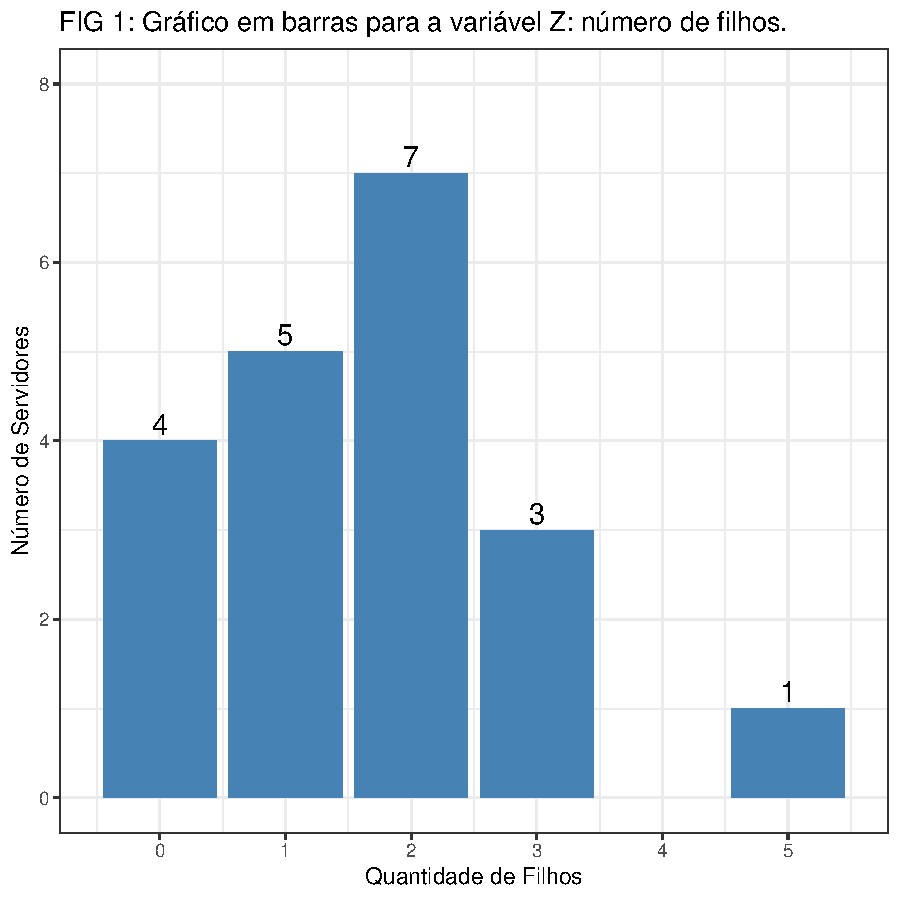
\includegraphics{Aula5-bar1}
\end{center}
\end{block}
\end{frame}
\subsection{Gráficos de Dispersão Unidimensionais}
\begin{frame}{}
\frametitle{Gráficos de Dispersão Unidimensionais}
\begin{block}{}
	\vspace{-0.5cm}
\begin{center}
\setkeys{Gin}{width=0.5\linewidth}
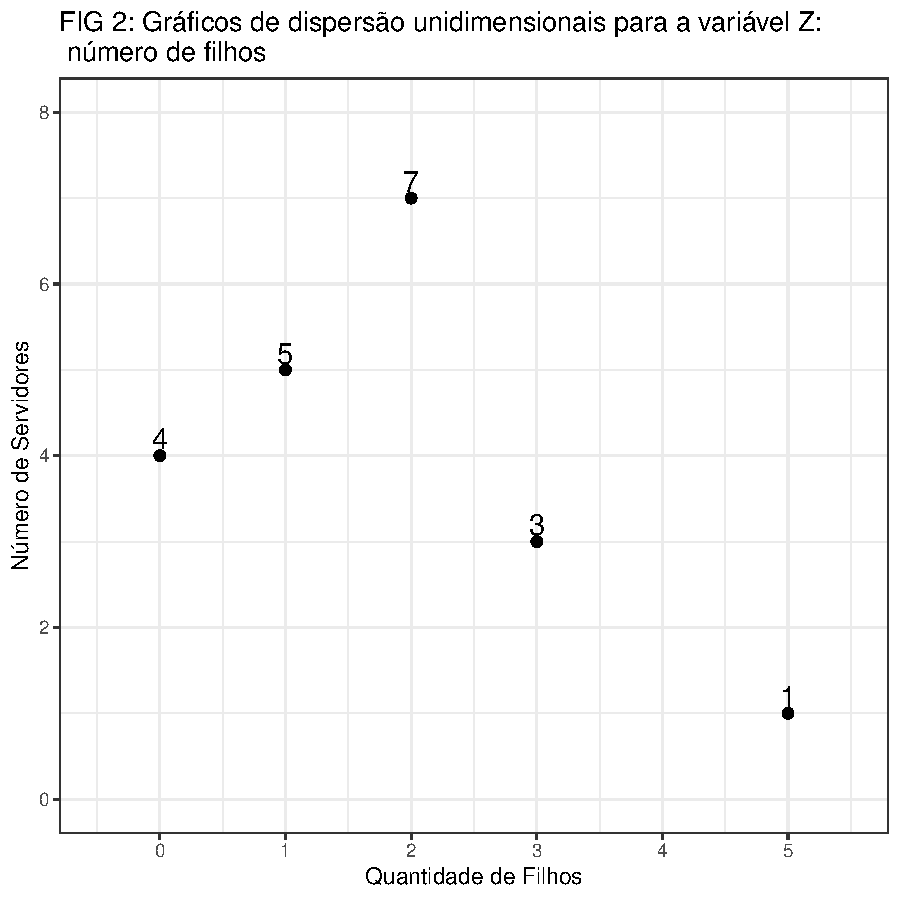
\includegraphics{Aula5-point1}
\end{center}
\end{block}
\end{frame}

\begin{frame}{}
\frametitle{Gráficos de Dispersão Unidimensionais}
\begin{block}{}
	\vspace{-0.5cm}
\begin{center}
\setkeys{Gin}{width=0.5\linewidth}
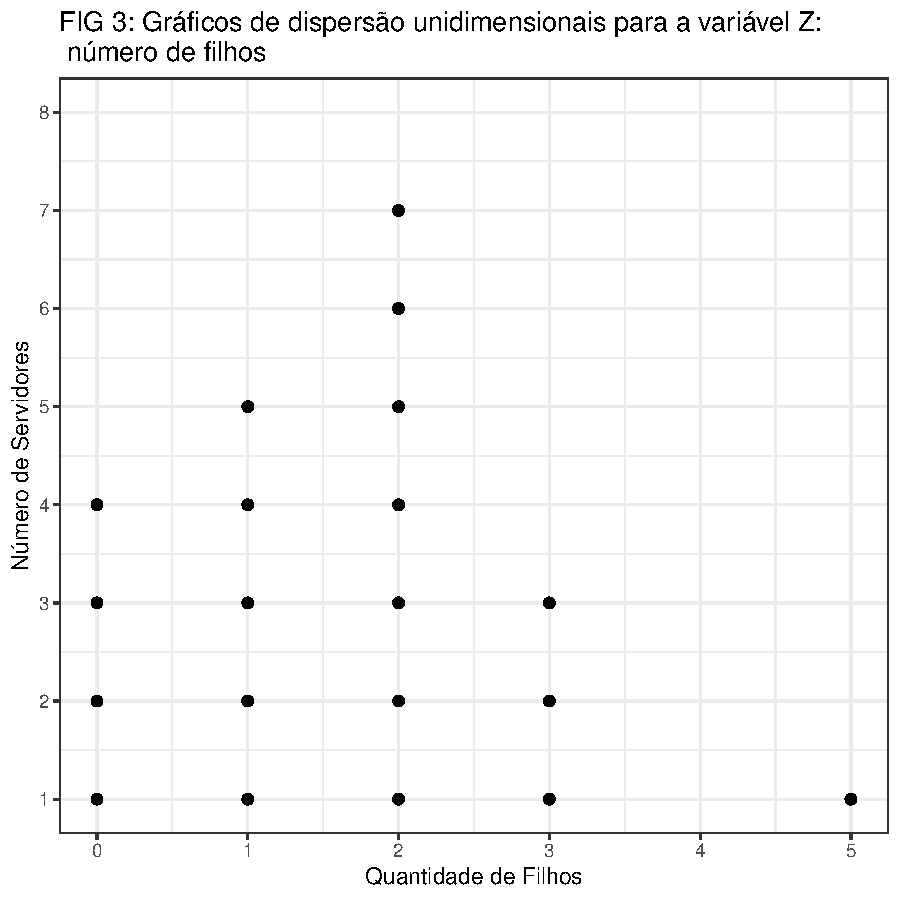
\includegraphics{Aula5-point2}
\end{center}
\end{block}
\end{frame}


\subsection{Histograma}
\begin{frame}{}
\frametitle{Histograma}
\begin{block}{}
\justifying
O histograma é um gráfico de barras contíguas, com as bases proporcionais aos intervalos
das classes e a área de cada retângulo proporcional à respectiva frequência. Pode-se
usar tanto a frequência absoluta, $f_{i},$ como a relativa, $f_{ri}.$
\end{block}
\end{frame}

\begin{frame}{}
\frametitle{}
\begin{block}{}
% \justifying
% \begin{figure}[H]
%     \centering
%     \includegraphics[scale=0.5]{Fig5}
%     \caption{Histograma da variável $S:$ Salários (\cite{Morettin09}).}
%     \label{Fig5_ex}
%   \end{figure}
\begin{center}
\setkeys{Gin}{width=0.5\linewidth}
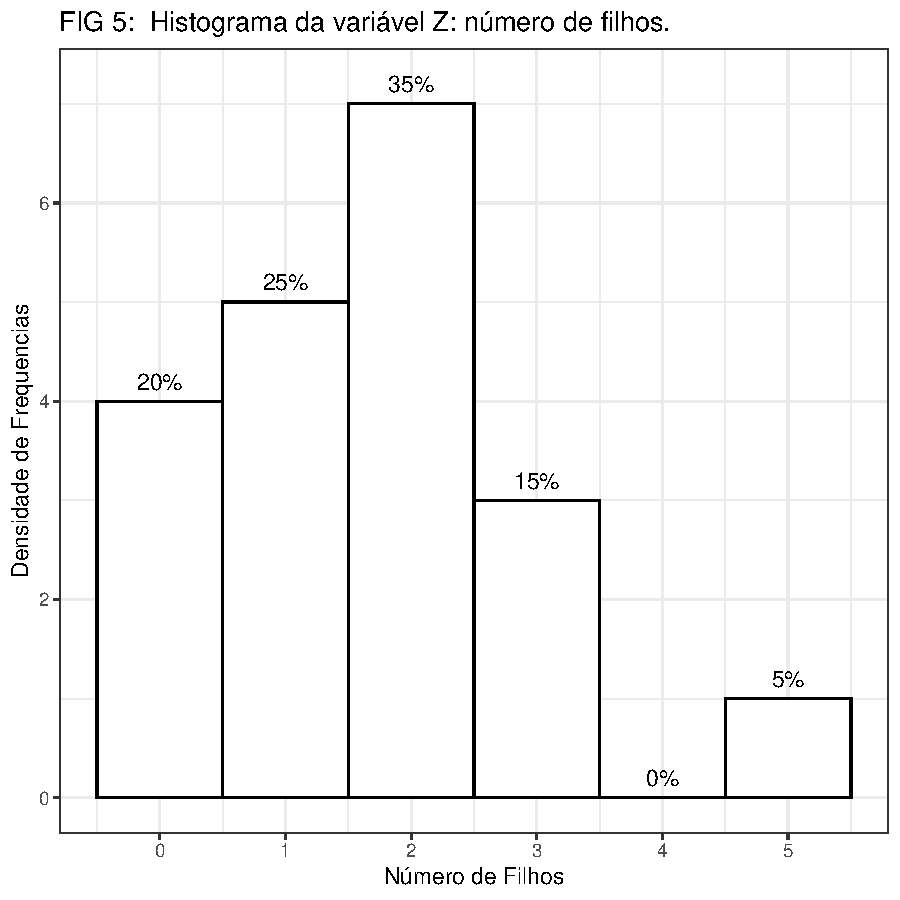
\includegraphics{Aula5-hist2}
\end{center}
\end{block}
\end{frame}

\begin{frame}{}
\frametitle{}
\begin{block}{}
\justifying
\begin{table}[H]
\caption{Frequências e porcentagens dos dos 36 empregados da seção de orçamentos da Companhia MB por faixa de salário.}
\label{tab4}
\begin{tabular}{c|c|c|c}
\hline
Classe de   &Ponto Médio&Frequência&Porcentagem\\
Salários    &    $S_{i}$& $n_{i}$  &$100f_{i}$ \\
\hline
~4.00|-~8.00&  6        &10        &27.78      \\
~8.00|-12.00& 10        &12        &33.33      \\
12.00|-16.00& 14        &8         &22.22      \\
16.00|-20.00& 18        &5         &13.89      \\
20.00|-24.00& 22        &1         & 2.78      \\
\hline
Total       &   $-$     &36        &100.00     \\
\hline
\end{tabular}
\subcaption*{\cite{Morettin09}}
\end{table}
\end{block}
\end{frame}

\begin{frame}{}
\frametitle{}
\begin{block}{}
% \justifying
% \begin{figure}[H]
%     \centering
%     \includegraphics[scale=0.5]{Fig5}
%     \caption{Histograma da variável $S:$ Salários (\cite{Morettin09}).}
%     \label{Fig5_ex}
%   \end{figure}
\begin{center}
\setkeys{Gin}{width=0.5\linewidth}
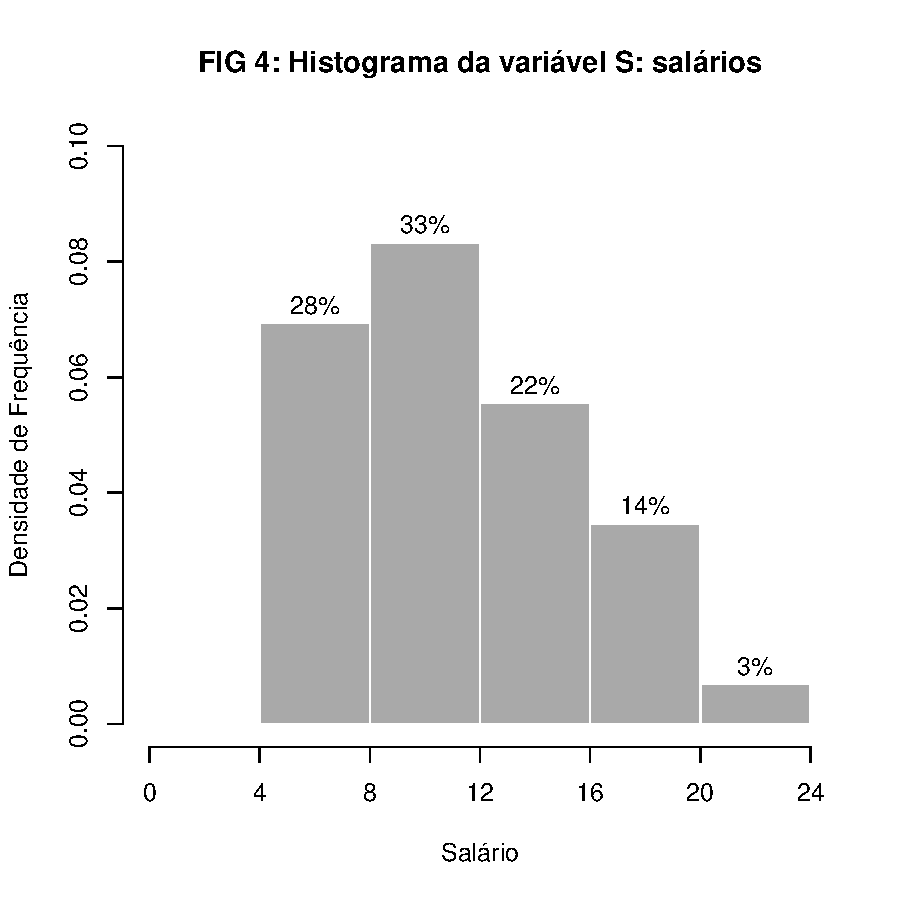
\includegraphics{Aula5-hist}
\end{center}
\end{block}
\end{frame}

\begin{frame}{}
\frametitle{Exemplo: Dados Fictícios}
\begin{block}{}
\begin{center}
\setkeys{Gin}{width=0.5\linewidth}
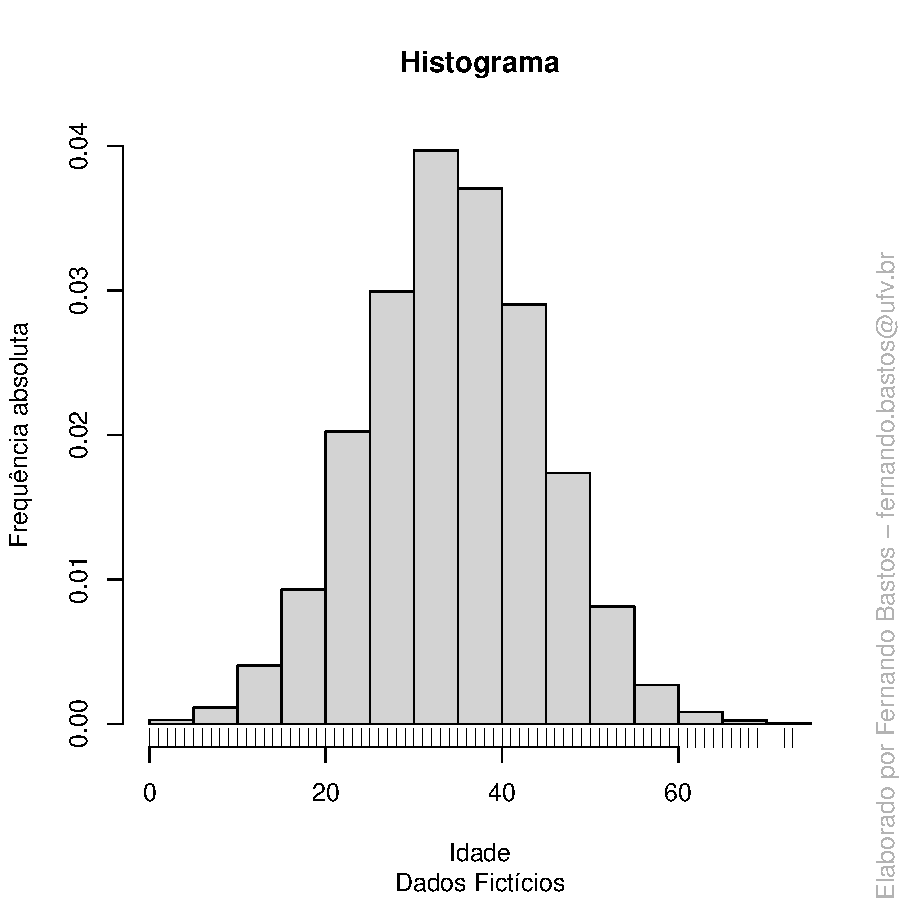
\includegraphics{Aula5-idade1}
\end{center}
\end{block}
\end{frame}

\subsection{Gráfico de Densidade}
\begin{frame}{}
\frametitle{Gráfico de densidade}
\begin{block}{}
\begin{center}
\setkeys{Gin}{width=0.5\linewidth}
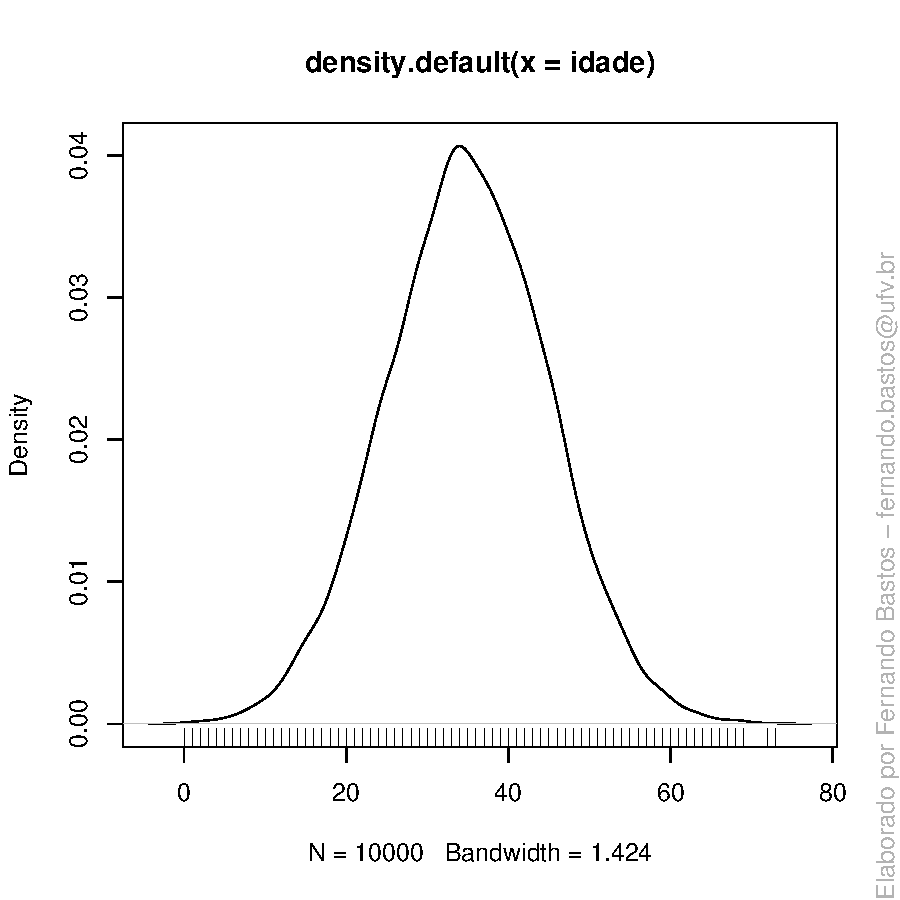
\includegraphics{Aula5-idade2}
\end{center}
\end{block}
\end{frame}

%\subsection{Gráfico de frequência acumulada empírica}
%\begin{frame}{}
%\frametitle{Gráfico de frequência acumulada empírica}
%\begin{block}{}
%\begin{center}
%\setkeys{Gin}{width=0.5\linewidth}
%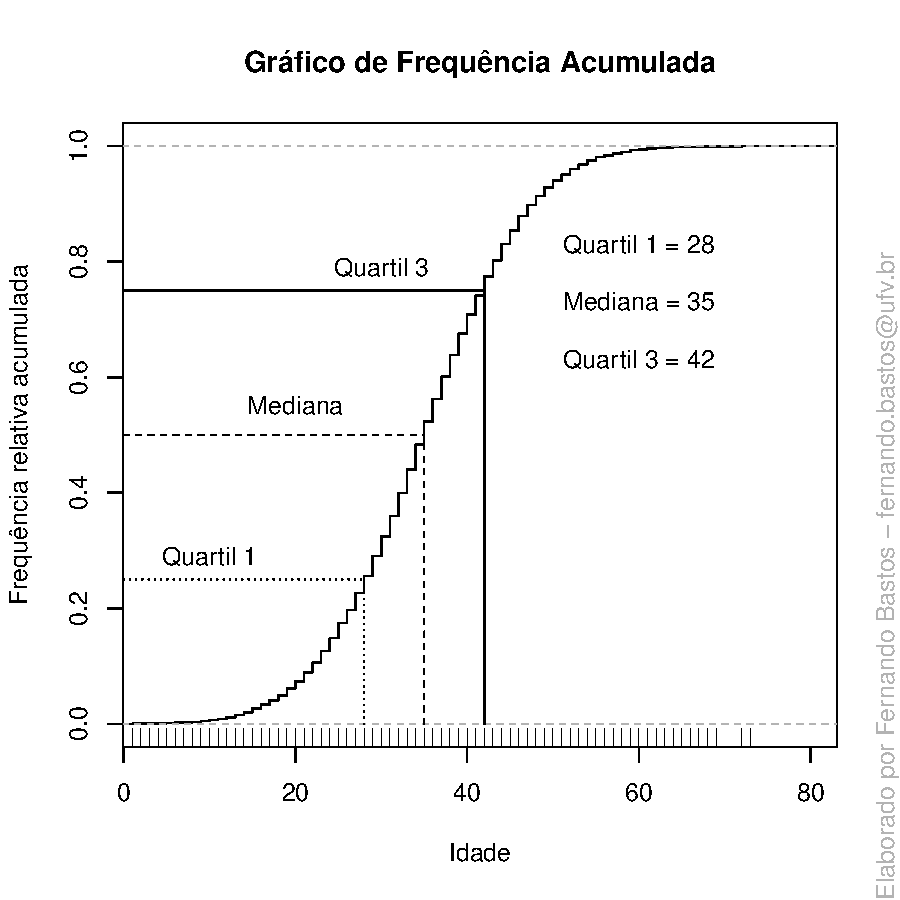
\includegraphics{Aula5-idade3}
%\end{center}
%\end{block}
%\end{frame}

\begin{frame}%[allowframebreaks]
\frametitle{\bf Referências}
\printbibliography
\end{frame}


\end{document}
